\chapter{Research methodology}\label{ch:research-methodology}

The research method used in this thesis follows the design science research (DSR) approach
\cite[p. 17]{rennenkampff_managementitagilitaetentwicklung_2015}.
DSR is a research paradigm in which the designer tries to create artifacts to answer questions
for problems.

% Pado: This still seems a little redundant and unclear - I feel your sources are not being very
% informative and you are unsure yourself of what they are trying to say.
% I would stick with the example from the literature  to explain what DSR is.

DSR is a research paradigm in which the designer creates artifacts and uses them to answer
questions for problems and generate new scientific knowledge.
The designed artifacts are both useful and fundamental to understanding the problem \cite[p.
10]{hevner_designscienceresearch_2010}

Design, according to Peffers et al. (2007), is the creation of an applicable solution to a
problem \cite[p.47]{peffers_designscienceresearch_2007}

According to Hevner et al. (2010)
design" is both a process ("a set of activities") and a product ("artifactt"). \cite[p
.78]{hevner_designscienceresearch_2010}
The design-oriented research approach as a methodological framework seems well suited to answer
the research questions.
Predicting spring back and bend deduction is a relevant problem in business practice.
Also, the conception and implementation of machine learning models is a design activity.

% Pado: Ah, this is where „Build“ comes from! I see. In that case, maybe quickly introduce DSR
% and its high-level phases in the Introduction to explain the naming choices in the thesis.

The term artifacts is intentionally broad and can take on different forms. In this work, the
artifact is different machine leaning models which are applied on the generated data.
DSR can be implemented in various ways, a prominent example is provided by Peffers et al. and
shown in Figure \ref{fig:dsr_process}
The approach comprises six steps, which are dived into the superordinate phases "Build" and
"Evaluate". This thesis follows these phases.

\begin{figure}[H]
    \begin{tcolorbox}[arc=0pt,boxrule=0.5pt]
        \centering
        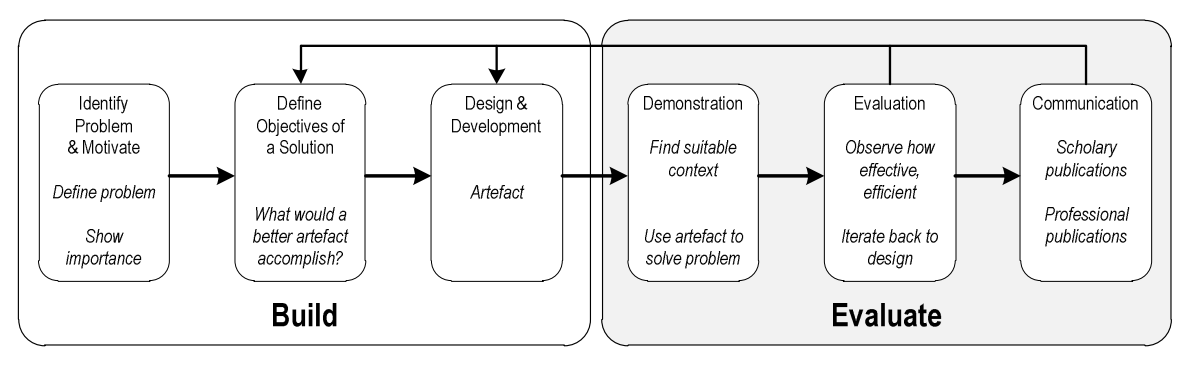
\includegraphics[width=1\linewidth]{chap3/images/dsr_process.png}
        \caption[DSR Process]{Design Science Research Approach according to Peffers et al.
        Picture: \cite[p. 72]{sonnenberg_evaluationpatternsdesign_2012}}
        \label{fig:dsr_process}
    \end{tcolorbox}
\end{figure}

% Pado: Can you make the approach even more concrete by relating each of the activities to your
% thesis? E.g., in the Design&Development step, the artefact is a machine learning model of
% springback and you will use training and optimisation strategies from ML in order to achieve a
% tool that can be shown to solve the problem in the Demonstration step and evaluated in the
% Evaluation step.

Also, I’m not quite clear on the distinction between Demonstration and Evaluation in your
context, since Demonstration would most likely be showing that your model predicts springback
reliably, which refers back to evaluation?

\paragraph{Activity 1 - Problem identification and motivation}
This activity includes defining a specific research problem and the value of a potential solution.
The problem is used for the development of the artifact. To reduce complexity, the problem should
be divided into sub-problems. For problem-solving, explicit methods such as system requirements
gathering or an implicit method such as programming and/or data analysis.
\cite[p. 52]{peffers_designscienceresearch_2007}

\paragraph{Activity 2: Define the objectives for a solution}
The goals of a solution are derived from the problem definition. These are derived in the context
of what is possible and feasible.
Objectives can be quantitative or qualitative. Objectives should be derived from the
problem specification and are thus based on the previous step.
For knowledge about previous solutions and their effectiveness are required
\cite[p. 55]{peffers_designscienceresearch_2007}

\paragraph{Activity 3: Design and development}
This step involves the creation of the artifact. An artifact can potentially contain models,
methods or constructs, it can be anything that contributes to the solution of the research question.
This step includes the definition of the functionality and architecture of the artifacts,
followed by the creation of them.
\cite[p. 55]{peffers_designscienceresearch_2007}

\paragraph{Activity 4: Demonstration}
The use of the previously created artifactt is demonstrated for one or more problems.
This requires effective knowledge of the artifact.
\cite[p. 55]{peffers_designscienceresearch_2007}
% Descripe what is done in this work 

\paragraph{Activity 5 - Evaluation}
It is observed and evaluated how well the developed artifact provides a solution to the defined
problems in activity 1.
Knowledge of relevant metrics and methods of analysis is assumed. Depending on the nature of the
problem, the evaluation can take different forms.
A comparison of the functionality of the artifact and other solutions can be considered.
Furthermore, quantified
quantified parameters can be used to measure the performance of the artifacts
\cite[p. 56]{peffers_designscienceresearch_2007}
Hevner et al. suggest five different evaluation methods: Observational
methods, analytical methods, experiments, testing of the artifact and descriptive
methods
\cite[p. 87]{hevner_designscienceinformation_2004}
% How is this work evaluated 

\paragraph{Activity 6 - Communication}
The problem and the artifactt and its benefit are communicated externally
\cite[p. 56]{peffers_designscienceresearch_2007}
Hevner et al. describe in a conceptual framework guidelines for the


\section{Design Principles}

% Pado: Do the principles guide the Design&Development step only, or are they used through the
% Build or even Build&Evaluate phases?
% Are there standard principles that should be used, or is there a set to choose from, or does
% one create them individually for each study?

Design Principles (DP) are seen as a central part of design-oriented research.
\cite[p. 348]{gregor_positioningpresentingdesign_2013}
Design principles are characterized as "principles of form and function" as well as "principles
of implementation" of an artifact.
\cite[p.8]{gregor_anatomydesigntheory_}
They are used to close the gap between researchers and user and allow prescriptive research on
systems. They are used to capture knowledge about the artifact.
\cite[pp. 37-56]{sein_actiondesignresearch_2011}.
Koppenhagen et al. suggest generating design principles by grouping requirements for the solution
and then creating core requirements, which can
which can then be DPs.
\cite[p. 6]{koppenhagen_designscienceresearch_2012}


\section{Evaluation of Machine Learning Models}\label{sec:evaluation-of-machine-learning-models}
Evaluating \ac{ML} models is different from evaluating other software artifacts for several reasons.
One of them is that data-driven software components, like \ac{ML} models, have functionality that
is not
completely defined by the developer but is
instead learned from data.
Therefore, using machine learning presents new challenges compared to traditional software
engineering~\cite[p. 2]{siebert2022construction}.

In the field of software engineering, there are already standards that define the quality of
software systems and its components.
Most notable the ISO/IEC 9126 standards, which provide a quality model which is widely adapted in
software engineering (Source).
For above-mentioned reasons these standards are not suitable to evaluate machine learning models,
therefore~\cite{siebert2022construction} note that they need to be adapted.
They re-interpreted and extended these existing quality models to the ML context~\cite[p.
1]{siebert2022construction}.

In order to define the Design Principles for the \ac{ML} models this work, the
considerations of~\cite[]{siebert2022construction} are used.
This enables a systematic process in order to assess the quality of the developed models.

In the work of~\cite{siebert2022construction}, several quality attributes are considered, including
Correctness, Relevance, Robustness, Stability, Interpretability and Resource
Utilization.
Alongside these attributes, the authors also provide a set of quality measures to evaluate the
models, but these are nor complete and are only used as a starting point for the evaluation of the
models in this work, further evaluation is described in Chapter~\ref{ch:evaluation}.

It is important to note, that the mentioned quality attributes and measures should
not be seen as a complete set of quality attributes and measures for \ac{ML} models.
Other studies, such as ~\cite{zhang2020machine} have proposed additional sets of quality attributes.
These additional perspectives will also be considered in the evaluation of the models, but only
as a supplementary means of evaluating model performance.

Attributes like Security, Fairness and Privacy~\cite[p. 3]{zhang2020machine} are not considered in
this work, as they are difficult to measure and my not be relevant for the use case of this work.


\section{Goal Question Metric Approach}\label{subsec:goal-question-metric-approach}
To make the defined quality attributes measurable, the “Goal-Question-Metric”-approach \ac{GQM}
was chosen in this work. It is one of the most common approaches in DSR and is divided into three
levels.
\cite[p. 3]{basili_goalquestionmetric_}

\paragraph{1. Conceptual level (goal):}
"A goal is defined for an object, for a variety of reasons,
with respect to various models of quality, from various points of view, relative to a
particular environment." \cite[p. 3]{basili_goalquestionmetric_}

\paragraph{2. operational level (question):}
"A set of questions is used to characterize the way
the assessment/achievement of a specific goal is going to be performed based on
some characterizing model. Questions try to characterize the object of
measurement (product, process, resource) with respect to a selected quality issue
and to determine its quality from the selected viewpoint." \cite[p. 3]{basili_goalquestionmetric_}

\paragraph{3. quantitative level (metric):}
"A set of data is associated with every question in order to answer it in a quantitative way."
\cite[p. 3]{basili_goalquestionmetric_}

Objectives, questions and metrics can be presented in a hierarchical structure.

\begin{figure}[H] % supposedly places it here ...
    \begin{tcolorbox}[arc=0pt,boxrule=0.5pt]
        \centering
        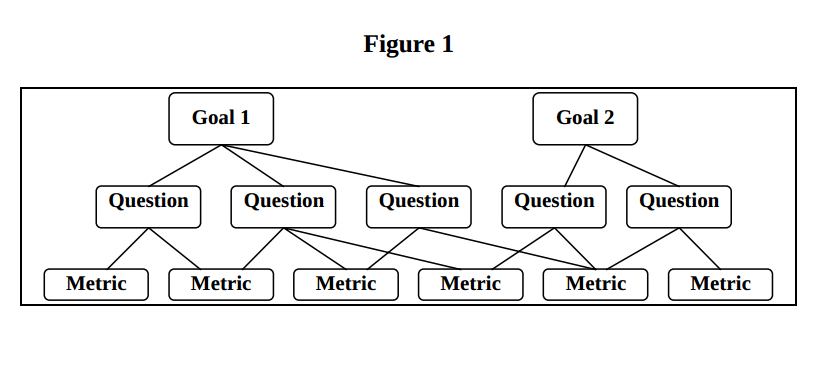
\includegraphics[width=0.8\linewidth]{gqm}
        \caption[GQM tree stucture ]{Goal-Question-Metric Ansatz \cite[p.
        3]{basili_goalquestionmetric_}}
        \label{fig:gqm}
    \end{tcolorbox}
\end{figure}
